\makeatletter
\def\input@path{{../styles/}{../../styles/}{../../../styles/}{../}{../../}{../../../}}
\makeatother
\documentclass{ee102_notes}
% macros.tex - Course meta information
\renewcommand{\course}{EE 102}
\renewcommand{\coursetitle}{Signal Processing and Linear Systems}
\renewcommand{\instructor}{Ayush Pandey}
\renewcommand{\semester}{Fall}
\renewcommand{\year}{2025}
\renewcommand{\shorttitle}{Week 1: Introduction to Signals}
% Use \renewcommand to avoid 'already defined' errors

% The following packages can be found on http:\\www.ctan.org
% \usepackage{graphics} % for pdf, bitmapped graphics files
%\usepackage{epsfig} % for postscript graphics files
%\usepackage{mathptmx} % assumes new font selection scheme installed
%\usepackage{times} % assumes new font selection scheme installed
\usepackage{amsmath} % assumes amsmath package installed
\usepackage{amssymb,mathtools}  % assumes amsmath package installed
\usepackage{xcolor}
\usepackage{pgfplots,subcaption}
\usepackage[hidelinks]{hyperref}
\usepackage{verbatim}
\usepackage{graphicx}
\usepackage{listings}

% -------- listings (Python) ----------
\lstdefinestyle{py}{
  language=Python,
  basicstyle=\ttfamily\small,
  keywordstyle=\color{blue!60!black}\bfseries,
  commentstyle=\color{green!40!black},
  stringstyle=\color{orange!60!black},
  showstringspaces=false,
  columns=fullflexible,
  frame=single,
  framerule=0.3pt,
  numbers=left,
  numberstyle=\tiny,
  xleftmargin=1em,
  tabsize=2,
  breaklines=true,
}
\usepackage[american]{circuitikz}
\usepackage{tikz}
\usepackage{caption}    
\usepackage{lscape}
\usepackage{soul}
\usepackage{tikz}
\usetikzlibrary{calc,angles,quotes,arrows.meta}

\usepackage{hyperref}
\hypersetup{
    colorlinks=true,
    linkcolor=blue,
    filecolor=magenta,      
    urlcolor=blue,
    pdftitle={week1_notes},
    pdfpagemode=FullScreen,
}
%\usepackage{float} 

%\usepackage[demo]{graphicx}
\pgfplotsset{compat=1.18}
% \usepgfplotslibrary{fillbetween}

\newsavebox{\measurebox}

\let\proof\relax\let\endproof\relax


\newcommand{\norm}[1]{\left\lVert#1\right\rVert}
\def\abs#1{\left\lvert#1\right\rvert}
\let\proof\relax
\let\endproof\relax
\usepackage{amsthm}
\usepackage{accents}
\usepackage{relsize}
\newcommand{\ubar}[1]{\underaccent{\bar}{#1}}
\newtheorem{theorem}{Theorem}
\newtheorem{corollary}{Corollary}[theorem]
\newtheorem{lemma}{Lemma}
\newtheorem{proposition}{Proposition}
\newtheorem{statement}{Statement}

\theoremstyle{definition}
\newtheorem{definition}{Definition}
 
\theoremstyle{remark}
\newtheorem*{remark}{Remark}
\theoremstyle{remark}
\newtheorem*{claim}{Claim}
\setlength{\parindent}{0cm}
\newenvironment{nalign}{
    \begin{equation}
    \begin{aligned}
}{
    \end{aligned}
    \end{equation}
    \ignorespacesafterend
}

\renewcommand{\releasedate}{November 12, 2025}
\newcommand{\Eblank}{\rule{3cm}{0.4pt}}
\newcommand{\Rankblank}{\rule{3cm}{0.4pt}}

\begin{document}
\section*{EE 102 Week 11, Lecture 2 (Fall 2025)}
\subsection*{Instructor: \instructor}
\subsection*{Date: \releasedate}
\section{Announcements}
\begin{itemize}
    \item HW \#10 will be due on Mon Nov 17.
    \item Rest of the semester: HW \#11 on Mon Nov 24, HW \#12 on Dec 8, Final exam on Dec 16 (Tue) from 9am to 11am.
    \item Dec 1: Guest Lecture by Prof. Xiaofan Yu on 2D Fourier Transforms and image processing applications. Dec 3: Guest lecture by Yaoyun Zhou on Fast Fourier Transform algorithms.
\end{itemize}

\section{Today's Learning Goals}
\begin{itemize}
    \item Understand frequency-selective filtering using the properties of Fourier analysis.
    \item Design ideal and realizable low-pass, high-pass, and band-pass filters.
\end{itemize}
\section{Low Pass Filters}
Filters are systems that take in an input signal and modify its frequency content to achieve a desired effect in the generated output. A low-pass filter is a system that allows low-frequency components to pass through while attenuating high-frequency components.
\begin{popquiz}
    Sketch a low-pass filter in the frequency domain.
    \popqsplit
    See Figure~\ref{fig:lowpass_filter-ideal}.
\end{popquiz}
We can sketch an ideal low-pass filter in the frequency domain with cutoff frequency \(\omega_c\) as a pulse shaped function between \(-\omega_c\) and \(\omega_c\):
\begin{figure}[h]
    \centering
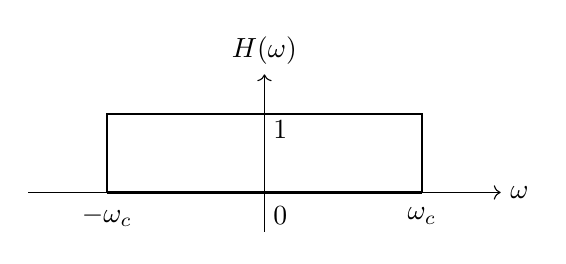
\begin{tikzpicture}
    \draw[->] (-3,0) -- (3,0) node[right] {$\omega$};
    \draw[thick] (-2,0) -- (2,0);
    \draw[thick] (-2,0) -- (-2,1) -- (2,1) -- (2,0);
    \node at (2,-0.3) {$\omega_c$};
    \node at (-2,-0.3) {$-\omega_c$};
    % y axis at 0:
    \draw[->] (0,-0.5) -- (0,1.5) node[above] {$H(\omega)$};
    % label 0 on x axis 0 on the right of the axis
    \node at (0.2,-0.3) {0};
    \node at (0.2, 0.8) {1};
\end{tikzpicture}
\caption{Ideal low-pass filter in the frequency domain.}
\label{fig:lowpass_filter-ideal}
\end{figure}
The low-pass filter in Figure~\ref{fig:lowpass_filter-ideal} allows frequencies below \(\abs{\omega_c}\) to pass through unchanged (because the magnitude of the frequency response is 1) while attenuating frequencies above \(\omega_c\) because the frequency response is 0. This is true because of the convolution property. 

The low-pass filter is an LTI system with frequency response $H_{\text{LP}}(\omega)$. It can be mathematically written as 
\[
H_{\text{LP}}(\omega) = \begin{cases}
    1, & |\omega| \leq \omega_c \\
    0, & |\omega| > \omega_c
\end{cases}
\]
or in other words, 
\[
H_{\text{LP}}(\omega) = \begin{cases}
    1, & \omega < \omega_c \land \omega > -\omega_c \\
    0, & \omega \geq \omega_c \lor \omega \leq -\omega_c
\end{cases}
\]
where $\land$ is the logical AND operator and $\lor$ is the logical OR operator. The passband is the range of frequencies that are allowed to pass through the filter without attenuation, while the stopband is the range of frequencies that are attenuated. In the case of the low-pass filter shown above, the passband is \(-\omega_c \leq \omega \leq \omega_c\) and the stopband is \(\omega < -\omega_c\) or \(\omega > \omega_c\).

Why does the filter turn the output 0 for frequencies outside the passband? This is where the convoltion property of Fourier analysis comes in --- one of the most important results that we have derived in this class! It says that the frequency response (the Fourier transform) of the output signal is equal to the multiplication of the frequency response of the input signal and the frequency response of the filtering system:
\[
Y(\omega) = X(\omega) \cdot H_{\text{LP}}(\omega)
\]
which, in the case of a low-pass filter, means that the frequency response of the output signal will be exactly equal to 0 for frequencies outside the passband and will pass the input as it is (without change) within the passband since the magnitude of the frequency response of the filter is 1 in the passband.

This is all great, but what about the time-domain representation of this filter? After all, anything that we will implement will be implemented in real-life systems where time response will be a consideration. So, we need to find the impulse response of the filter, $h_{\text{LP}}(t)$, which is the inverse Fourier transform of $H_{\text{LP}}(\omega)$.

Applying the inverse Fourier transform, we get:
\[
h_{\text{LP}}(t) = \frac{1}{2\pi} \int_{-\infty}^{\infty} H_{\text{LP}}(\omega) e^{j \omega t} d\omega = \frac{1}{2\pi} \int_{-\omega_c}^{\omega_c} e^{j \omega t} d\omega
\]
Evaluating the integral, we have:
\[
h_{\text{LP}}(t) = \frac{1}{2\pi} \left[ \frac{e^{j \omega t}}{j t} \right]_{-\omega_c}^{\omega_c} = \frac{1}{2\pi j t} \left( e^{j \omega_c t} - e^{-j \omega_c t} \right)
\]
Using Euler's formula, this simplifies to:
\[
h_{\text{LP}}(t) = \frac{\sin (\omega_c t)}{\pi t}
\]
Let us plot the impulse response to understand the ideal low-pass filter in the time domain.
\begin{figure}[h]
    \centering
    \begin{tikzpicture}
        \draw[->] (-4,0) -- (4,0) node[right] {$t$};
        \draw[->] (0,-1.5) -- (0,2) node[above] {$h_{\text{LP}}(t)$};
        % Plot the sinc function
        \draw[thick, black, domain=-4:4, samples=100] plot (\x, {sin(deg(4.5*\x))/(pi*\x)});
    \end{tikzpicture}
    \caption{Impulse response of the ideal low-pass filter.}
    \label{fig:impulse_response_ideal_lowpass}
\end{figure}
From Figure~\ref{fig:impulse_response_ideal_lowpass}, we can observe that it extends for all time: $(-\infty, \infty)$. But the intuition behind ``low-passing'' is not quite apparent just from the time-domain. What about the computation of the output of the system, $y(t)$? We know that the output of an LTI system in time-domain is given by the convolution integral. So, we can compute $y(t)$ as
\[
y(t) = x(t) * h_{\text{LP}}(t) = \int_{-\infty}^{\infty} x(\tau) h_{\text{LP}}(t - \tau) d\tau
\]
On the other hand, the frequency response of the output is given by the product of the frequency responses of the input and the filter:
\[
Y(\omega) = X(\omega) \cdot H_{\text{LP}}(\omega)
\]
It is clear that in the frequency domain the output is easily computed by multiplication, which is often simpler than convolution in the time domain. But the time-domain does reveal three ``problems'' with the ideal low-pass filter:
\begin{enumerate}
    \item The impulse response $h_{\text{LP}}(t)$ is not zero for $t < 0$. This means that the ideal low-pass filter is non-causal and therefore, it cannot be implemented in real-time systems.
    \item The impulse response extends infinitely in time, which means the filter has an infinite duration impulse response and is not time-limited. Not practical for real-time implementation.
    \item We observe a ring-y behavior in the impulse response. Notice the trailing oscillations --- these are a direct result of the sharp cut-off in the frequency domain. In fact, as you would recall, the sharp cutoff is a negative impulse and impulse signal is made up of all frequencies from $-\infty$ to $\infty$. So, we get the Gibbs phenomenon which show up as oscillations in the time domain.
\end{enumerate}
Why are oscillations a problem? A common application of low-pass filtering is in automotives --- design of suspension systems. The bumps and jerks that you feel on the road (if your suspension systems are not perfect) are high frequency signals. So, suspension systems are designed on the concept of a low-pass filter that smooths out these high frequency disturbances, providing a more comfortable ride. If the ideal low-pass filter is used with ring-y impulse response, we observe that the output will have oscillations (due to Gibbs phenomena) that can cause discomfort and instability in the system, defeating the purpose of the suspensions. So, we discuss non-ideal, realizable filter designs next.

\section{Realizable Low-pass Filters}
We have discussed a real-life low-pass filter before: the RC circuit. It is a simple example of a first-order low-pass filter that is causal (addressed the first issue above) and has an exponentially decaying impulse response, which is more practical for real-time implementation.

Recall that the impulse response of an RC circuit is given by 
\[
h_{\text{RC}}(t) = \frac{1}{RC} e^{-\frac{t}{RC}} u(t)
\]
where $u(t)$ is the unit step function, ensuring causality. Let's substitute $1/RC = a$ for simplicity. Then, the impulse response becomes
\[
h_{\text{RC}}(t) = a e^{-a t} u(t)
\]
The frequency response of this filter can be found by taking the Fourier Transform of the impulse response:
\[
H_{\text{RC}}(\omega) = \int_{-\infty}^{\infty} h_{\text{RC}}(t) e^{-j \omega t} dt = \int_0^{\infty} a e^{-a t} e^{-j \omega t} dt
\]
which can be evaluated as
\[
H_{\text{RC}}(\omega) = \int_0^{\infty} a e^{-(a + j \omega) t} dt = \frac{a}{a + j \omega}
\]

\begin{popquiz}
    By computing the magnitude of the frequency response, comment on what happens when $\omega \to 0$ and when $\omega \to \infty$.
    \popqsplit 
    We see that as $\omega \to 0$, the magnitude approaches 1, and as $\omega \to \infty$, the magnitude approaches 0.
\end{popquiz}
\subsection{The cut-off frequency and bandwidth}
This frequency response shows that the RC circuit acts as a low-pass filter because as $\omega \to 0$, the magnitude approaches 1, and as $\omega \to \infty$, the magnitude approaches 0. You can see this by evaluating the magnitude response
\[
|H_{\text{RC}}(\omega)| = \frac{a}{\sqrt{a^2 + \omega^2}}
\]
which decreases as $\omega$ increases, confirming the low-pass behavior. Let's sketch this frequency response and compare it with the ideal low-pass filter on the same sketch. See Figure~\ref{fig:impulse_response_comparison}.
\begin{figure}[h]
    \centering 
    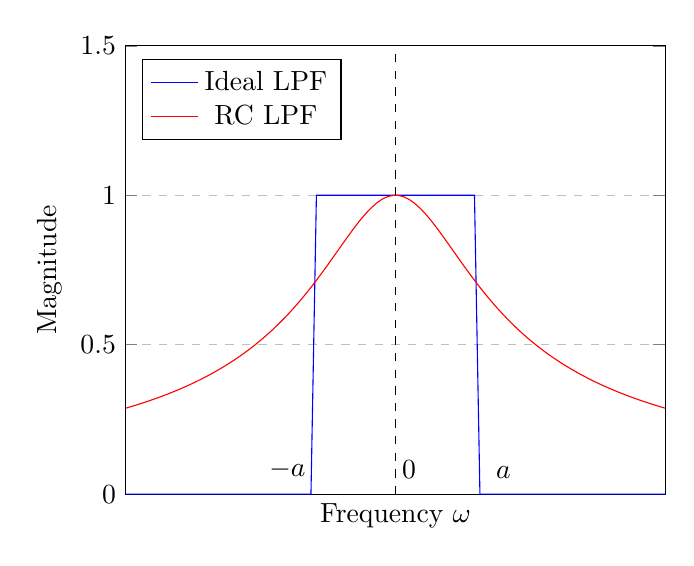
\begin{tikzpicture}
    \begin{axis}[
        xlabel={Frequency $\omega$},
        ylabel={Magnitude},
        xmin=-10, xmax=10,
        ymin=0, ymax=1.5,
        legend pos=north west,     % legend top-right
        ymajorgrids=true,
        grid style=dashed,
        xtick=\empty,              % hide x-axis tick marks and labels
    ]

    % Ideal low-pass filter
    \addplot[domain=-10:10, samples=100, color=blue]
        {abs(x) < 3 ? 1 : 0};
    \addlegendentry{Ideal LPF}

    % RC low-pass filter
    \addplot[domain=-10:10, samples=100, color=red]
        {3 / sqrt(9 + x^2)};
    \addlegendentry{RC LPF}

    \node[anchor=south] at (axis cs:-4,0.02) {$-a$};
    \node[anchor=south] at (axis cs: 4,0.02) {$a$};
    % mark the vertical y-axis at 0
    \node[anchor=south] at (axis cs:0.5,0.02) {0};
    % draw vertical line at 0 dashed
    \draw[dashed] (axis cs:0,0) -- (axis cs:0,1.5);
    \end{axis}
    \end{tikzpicture}

    \caption{Comparison of the magnitude response of the ideal low-pass filter and the RC low-pass filter. The cut-off frequency of the ideal filter is at $\omega = a$.}
    \label{fig:impulse_response_comparison}
\end{figure}

Find out the value of the RC low-pass filter at $\omega = a$ and $\omega = -a$. We have 
\[
|H_{\text{RC}}(a)| = |H_{\text{RC}}(-a)| = \frac{a}{\sqrt{a^2 + a^2}} = \frac{a}{\sqrt{2a^2}} = \frac{1}{\sqrt{2}} \approx 0.707
\]
This has been given a special name and is treated as the unique point called the \textit{cut-off frequency} or \textit{3 dB point} of the filter, where the output power drops to half of the input power (the frequency response therefore drops by 1 over the square root of 2 --- remember Parseval's theorem).

So, the cut-off frequency of the RC filter is defined to be at \(\omega_c = a = \frac{1}{RC}\). This also defines the bandwidth of the filter. In this case, the bandwidth is \(\omega_c\).

\section{High-pass and Band-pass Filters}
We can design other filters from the low-pass filter by using Fourier transform properties. First, let us create a high-pass filter from the low-pass filter by applying a frequency shift and inversion. The frequency response of a high-pass filter can be expressed as
\[
H_{\text{HP}}(\omega) = 1 - H_{\text{RC}}(\omega) = 1 - \frac{a}{a + j \omega} = \frac{j \omega}{a + j \omega}
\]
This filter attenuates low frequencies and allows high frequencies to pass, which is the opposite behavior of the low-pass filter. See Figure~\ref{fig:mag-high-pass}.
\begin{figure}
    \centering
    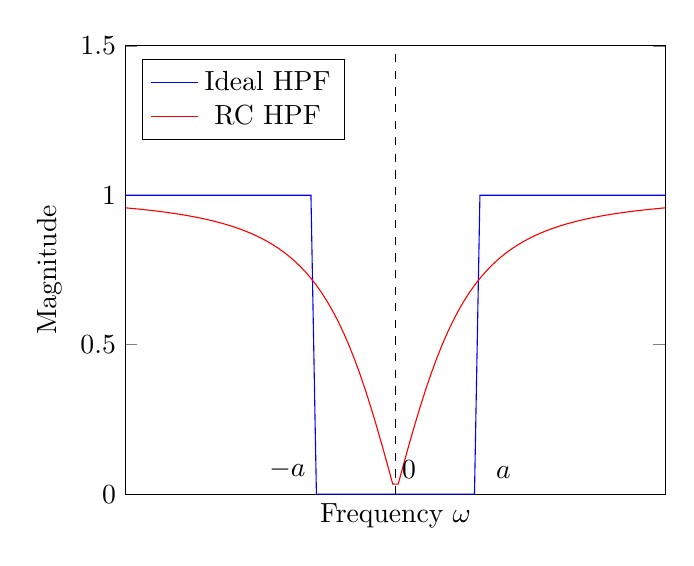
\begin{tikzpicture}
        \begin{axis}[
            xlabel={Frequency $\omega$},
            ylabel={Magnitude},
            xmin=-10, xmax=10,
            ymin=0, ymax=1.5,
            legend pos=north west,
            xtick=\empty,
        ]
        \addplot[domain=-10:10, samples=100, color=blue]
            {abs(x) > 3 ? 1 : 0};
        \addlegendentry{Ideal HPF}
        \addplot[domain=-10:10, samples=100, color=red]
            {abs(x) / sqrt(9 + x^2)};
        \addlegendentry{RC HPF}
        \node[anchor=south] at (axis cs:-4,0.02) {$-a$};
        \node[anchor=south] at (axis cs: 4,0.02) {$a$};
        % mark the vertical y-axis at 0
        \node[anchor=south] at (axis cs:0.5,0.02) {0};
        % draw vertical line at 0 dashed
        \draw[dashed] (axis cs:0,0) -- (axis cs:0,1.5);
 
        \end{axis}
    \end{tikzpicture}
    \caption{Comparison of the magnitude response of the ideal high-pass filter and the RC high-pass filter. The cut-off frequency of the ideal filter is at $\omega = a$.}
    \label{fig:mag-high-pass}
\end{figure}

Similarly, a band-pass filter can be created by combining a low-pass and a high-pass filter, allowing frequencies within a certain range to pass while attenuating frequencies outside that range. The design and analysis of these filters follow from the properties of their frequency responses.

By using Fourier transform properties, we can design other filters. Recall that a frequency shift is a multiplication by complex exponential:
\[
\mathcal{F}\{x(t)e^{j\omega_\ell t}\}=X(\omega-\omega_\ell),
\qquad
\mathcal{F}\{x(t)e^{-j\omega_\ell t}\}=X(\omega+\omega_\ell).
\]

Consider a signal \(x(t)\) with Fourier Transform \(X(\omega)\). Now, we desire a new ``frequency-selective'' filter where we can tunably pick a frequency band that the filter passes. Let us call this tunable frequency \(\omega_\ell\). 

We start by considering a frequency shift in the original signal to obtain: \(y(t)=x(t)e^{j\omega_\ell t}\Rightarrow Y(\omega)=X(\omega-\omega_\ell)\). Then, if you pass $y(t)$ through the ideal low-pass filter we discussed above, we get \(w(t)=y(t)*h(t)\Rightarrow W(\omega)=H(\omega)X(\omega-\omega_\ell)\).
Finally, if you shift back, you get \(f(t)=w(t)e^{-j\omega_\ell t}\Rightarrow F(\omega)=W(\omega+\omega_\ell)\).

This cascade implements a band-pass filter that is now centered at \(\omega_\ell\) using a fixed low-pass filter and two modulators. The pipeline is ``shift frequency by tunable amount \(\to\) select the band using the low-pass \(\to\) shift back'' (see Section 4.5.1 in Oppenheim and Willsky for more details). See Figure~\ref{fig:freq-selective-filter} for a visual illustration.
\begin{figure}[ht]
    \centering
    \includegraphics[width=\textwidth]{frequency_selective_filtering.png}
    \caption{Frequency-selective filtering process: shifting the spectrum $X(\omega)$ to get $Y(\omega)$, applying a low-pass filter to get $W(\omega)$, and shifting back to obtain a band-pass filter centered at \(\omega_\ell\), $F(\omega)$.}
    \label{fig:freq-selective-filter}
\end{figure}
\section{Frequency-selective Filter Design}


Therefore, with the same low-pass filter as above and not changing anything in it, we were able to obtain a band-pass filter by carefully applying the shifts in the frequency domain! The overall operation is still a linear and time-invariant system.

\section{Recommended Reading}
The content of this lecture is directly applicable to the design of amplitude modulation systems. Here are two solved examples that you should work on to make sure you understand the concepts thoroughly:
\begin{enumerate}
    \item Solved Example 4.21 in \textit{Signals and Systems} by Oppenheim and Willsky 2nd Edition
    \item Solved Example 4.22 in \textit{Signals and Systems} by Oppenheim and Willsky 2nd Edition
\end{enumerate}

\end{document}